\chapter{Presentación del problema y análisis de requisitos.}
\epigraphhead [30]{%
  \epigraph{``Los problemas son oportunidades para demostrar lo que se sabe."}%
  {Duke Ellington, compositor y músico.}%
}

En este capítulo se presentan los problemas de las soluciones actuales y la nueva propuesta para solventarlos. También se analizan los requisitos que ha de cumplir la nueva solución para que realmente sea una alternativa viable.
\section{Problemas de la solución actual.}
Ambas soluciones actuales son totalmente funcionales pero no libres de problemas e inconvenientes especialmente económicos que han motivado a la realización de este proyecto. A continuación se enumeran detalladamente para cada una de ellas:

\section*{Pasco 500 Interface}
\begin{itemize}
	\item El coste del interfaz es de unos 600€, aunque a esto habría que añadirle el coste del software para su manejo.
	\item Necesita de un equipo para poder usarse, puede ser un equipo con Windows pero el software para dicho sistema operativo impone ciertas limitaciones que hacen optar al departamento por adquirir equipos Apple, con el sobrecoste añadido.
\end{itemize}
\section*{Nucleus Personal Computer Analyzer II}
\begin{itemize}
	\item El material disponible actualmente está totalmente obsoleto (los documentos más recientes que disponemos datan de 1990).
	\item El reemplazo de dicho material bien por avería o por obsolescencia tiene un coste de aproximadamente 2000€ y un nuevo computador.
	\item Los computadores con los que puede funcionar la actual solución han de ser equipos que soporten MS-DOS y tengan puertos ISA para conectar las tarjetas de adquisición. Estos equipos en el mejor de los casos tienen diez años de antigüedad y la mayoría están alcanzando el final de su vida útil.
\end{itemize}

	El principal desafío de este proyecto es realizar una solución cuya diferencia de coste sea muy inferior a las actuales.

\section{Análisis de requisitos.}
		Heredado de las soluciones actuales, se pueden definir los siguientes requisitos mínimos para nuestro sistema final.
	\begin{itemize}
		\item{Representación de medidas en tiempo real. }El software debe proporcionar la posibilidad de leer en tiempo real el estado de las medidas, bien en una lectura digital o en una gráfica temporal.
		\item{Manejo de las medidas. }Para poder utilizar las medidas tomadas eficientemente, se deberá proveer la manera de combinar unas con otras, de manera que se puedan tomar medidas compuestas donde dos o más medidas se contrasten (por ejemplo, gráficas Temperatura-Presión). Estas gráficas y tablas deben ser posibles de almacenar para su posterior uso. Por supuesto, estas gráficas deben tener la posibilidad de ampliar, reducir y tomar captura de los datos representados.
		\item{Exportación de datos. }Los datos tomados con la aplicación deben poder ser exportados a otros formatos para su manipulación. Por ejemplo en formato de datos separados por comas (\emph{character-separated values} o CSV) para las tablas y \emph{portable network graphics} (PNG) para las gráficas o histogramas.
		\item{Guardar sesión. }El programa debe permitir guardar el estado actual para poder continuar en otro momento o sesión, o incluso para que el alumno pueda en su casa revisar el trabajo hecho en el laboratorio. También es una manera de realizar plantillas para los diversos experimentos que se realizarán.
		\item{Posibilidad de realizar medidas programadas.} Esto es, el software se programa para que realice una medida a uno o más sensores durante un tiempo determinado.
		\item{Posibilidad de realizar cálculos con las medidas tomadas. }Para ciertos experimentos puede ser interesante realizar automáticamente ciertos cálculos matemáticos más o menos complejos. La automatización de esta tarea puede suponer una ayuda para el alumno y el profesor.
	\end{itemize}


\section{Solución propuesta.}

\subsection{Sistema base.}
Desde que el proyecto era solo una idea, la intención ha sido utilizar una SBC (\emph{Single-board computer}) \emph{Raspberry Pi} para realizar la solución. No obstante, se investigaron otras posibilidades y su viabilidad: La \emph{Raspberry Pi} es un SBC económico pero muy básico y poco potente, por lo que el objetivo del búsqueda era algo más completo y potente. 

La \emph{Intel Galileo} fue una de las placas, descartada por no tener conexión a un monitor y porque según opiniones encontradas en internet, no resultaba ser tan potente como \emph{Intel} daba a entender. No obstante se barajó la posibilidad de poder usarse como equipo de procesamiento que realizara tareas complejas y liberara de carga al sistema principal ya que realmente su utilidad es más similar a la de las placas \emph{Arduino}. 

Éstas también fueron tomadas en cuenta y por la misma razón que las \emph{Galileo} fueron descartadas. No obstante, se consideró igualmente la utilización de la misma como por ejemplo convertidor analógico digital y descargar a la \emph{Raspberry Pi} de computación extra (por ejemplo, descartando datos no válidos u operando con ellos para dar datos precocinados al software final).

Por otra parte están las placas que se lanzaron posteriormente como respuesta al éxito de la Raspberry Pi. Una de ellas, la Cubieboard con una potencia en general superior y varias versiones con diferentes características y, naturalmente, un precio superior partiendo de los 50€.

Otra de ellas es la Banana Pi, se describe como un clon de la Raspberry Pi pero más potente. En efecto, con un precio ajustado de solo 50€ supera en características incluso a la Cubieboard, ofreciendo un procesador con dos núcleos más moderno, 1GB de memoria RAM y misma conectividad que la Raspberry.

%\pagebreak
\begin{savenotes}
\begin{table}[!ht]
  \centering
  \begin{tabular}{| c | c | c | c | c | c |}
  	\hline
    Nombre & Procesador & RAM & USB & Salida de vídeo & I/O \\ \hline
    \bigcell{c}{Raspberry Pi \\ Model B} & \bigcell{c}{ARMv6 \\ 700MHz} & 512MB & Sí & \bigcell{c}{HDMI, VGA, \\ Composite} & \bigcell{c}{GPIO, I\ts{2}C, \\ SPI}\\ \hline
    Arduino Uno\footnote{En combinación con otro SBC.} & \bigcell{c}{ATmega328 \\ 16 MHz} & 2KB & No &  No & Serial, SPI \\ \hline
    Intel Galileo & \bigcell{c}{Intel Quark \\ X1000 (x86) \\ 400 MHz} & 256MB & Sí & No & \bigcell{c}{Serial, UART,\\ ACPI, PCIe} \\  \hline
    Cubieboard1 & \bigcell{c}{Cortex-A8 \\ 1 GHz} & 1GB & Sí & HDMI & I\ts{2}C, SPI, LVDS \\ \hline
    Banana Pi & \bigcell{c}{Cortex-A7 \\ Dual core} & 1GB & Sí & \bigcell{c}{HDMI \\ Composite} & \bigcell{c}{GPIO, I\ts{2}C, \\ SPI} \\ \hline
  \end{tabular}
  \caption{Los diferentes SBC comparados.}
  \label{tab:sbc_compare}
\end{table}
\end{savenotes}

	Al final nos decidimos por mantener la idea original. Aunque las alternativas Cubieboard o Banana Pi son interesantes por su potencia extra, la comunidad tras de ellas es prácticamente inexistente, justo al contrario que con la \emph{Raspberry Pi}, la cual goza de una cantidad de soporte en internet enorme y eso hace más sencilla la tarea de solucionar problemas, buscar librerías o recabar experiencias. Además del reducido coste de la Raspberry Pi, factor a tener en cuenta dados los objetivos del proyecto. 


\subsection{Software y sistema operativo.}
	La Raspberry pi ofrece como sistemas operativos las siguientes opciones: \emph{GNU/Linux} (varias distribuciones) o \emph{RISC OS}. La decisión es una distribución \emph{GNU/Linux}, en este caso \emph{Raspbian}(\autoref{fig:raspbian-desktop}), una versión portada de \emph{Debian 7.0 Wheezy} a la \emph{Raspberry Pi} con mayor comunidad y desarrollo detrás respecto a otras opciones como \emph{Arch Linux} o \emph{pidora} (versión portada de \emph{Fedora} a Raspberry Pi).

	La siguiente decisión es qué lenguaje o lenguajes de programación se utilizarán para desarrollar el software necesario para hacer que la solución funcione. Después de cursar toda la carrera a uno siempre le viene a la cabeza el mismo lenguaje de programación: Java. Es el lenguaje que más se estudia y más a fondo en todo el programa académico, por tanto la familiarización con el mismo es muy alta, pero nuestra SBC tiene una potencia relativamente limitada y operar la máquina virtual de Java sobre ella traería más quebraderos de cabeza que beneficios. \emph{C} es una opción relativamente viable, su bajo nivel y rendimiento es adecuado para lo que se desea desarrollar, pero es un lenguaje especialmente complicado y en el que sin experiencia adecuada el proceso se puede complicar rápidamente.
	
	La comunidad de la Raspberry Pi tiene especial predilección por \emph{Python}, siendo uno de los lenguajes que te invitan a aprender -junto a otros- con tu nueva unidad e instalación de \emph{Raspbian}. Pese a tener alguna noción básica del lenguaje procedentes de la asignatura \emph{Procesadores del Lenguaje}, realizar el proyecto ha sido llevar mis conocimientos de este lenguaje a otro nivel completamente distinto, añadiendo dificultad extra ya que el aprendizaje del  mismo se ha realizado \emph{``al vuelo"} a la vez que se ha desarrollado, y esto ha inducido a errores sobre todo en las estructuras internas y funciones de \emph{Python} de programación.

\begin{figure}[hb]
  \centering
  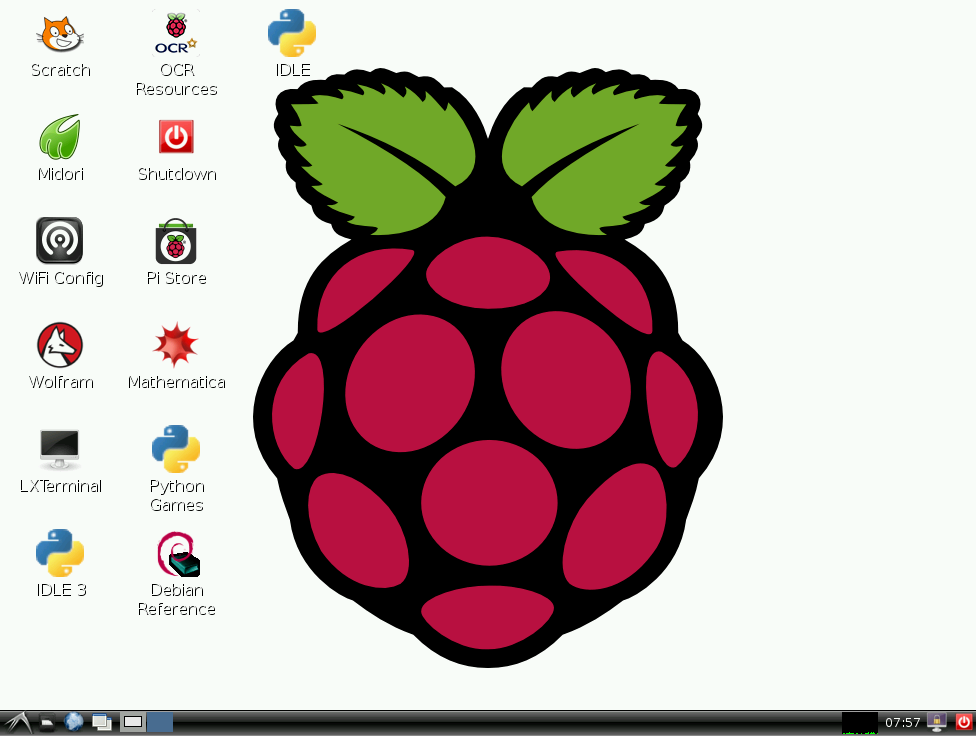
\includegraphics[width=1\textwidth]{img/2014-08-22-075744_976x736_scrot.png}
  \caption[Escritorio de Raspbian.]{Raspbian.}
  \label{fig:raspbian-desktop}
\end{figure}